\documentclass[10pt]{article}
\usepackage[polish]{babel}
\usepackage[utf8]{inputenc}
\usepackage[T1]{fontenc}
\usepackage{amsmath}
\usepackage{amsfonts}
\usepackage{amssymb}
\usepackage[version=4]{mhchem}
\usepackage{stmaryrd}
\usepackage{graphicx}
\usepackage[export]{adjustbox}
\graphicspath{ {./images/} }
\usepackage{bbold}

\title{PRACA KONTROLNA nr 1 - POZIOM PODSTAWOWY }

\author{}
\date{}


\begin{document}
\maketitle
\begin{enumerate}
  \item Właściciel hurtowni sprzedał $\frac{1}{3}$ partii bananów po założonej przez siebie cenie. Okazało się, że owoce zbyt szybko dojrzewają, więc obniżył cenę o $30 \%$ i wówczas sprzedał $60 \%$ pozostałej ilości owoców. Resztę bananów udało mu się sprzedać dopiero, gdy ustalił ich cenę na poziomie $\frac{1}{5}$ ceny początkowej. Ile procent zaplanowanego zysku stanowi kwota uzyskana ze sprzedaży? Po ile powinien był sprzedać pierwszą partię towaru, by jednokrotna obniżka ich ceny o $25 \%$ pozwoliła na sprzedaż wszystkich owoców i uzyskanie zaplanowanego początkowo zysku?
  \item Przekątne trapezu o podstawach 3 i 4 przecinają się pod kątem prostym. Na każdym z boków trapezu, jako na średnicy, oparto półokrąg. Obliczyć sumę pól otrzymanych czterech półkoli. Sporządzić rysunek.
  \item Uprościć wyrażenie $\frac{1}{\sqrt{a}-\sqrt{b}}\left(\sqrt[6]{a^{5}}-\frac{b}{\sqrt[6]{a}}\right)-\frac{a-b}{\sqrt[3]{a^{2}}+\sqrt[6]{a} \sqrt{b}}$ dla $a, b$, dla których ma ono sens. Następnie obliczyć jego wartość, przyjmując $a=(4-2 \sqrt{3})^{3}$ i $b=3+2 \sqrt{2}$.
  \item Podstawą ostrosłupa prawidłowego jest sześciokąt foremny o boku $a$. Obliczyć objętość, wiedząc, że najmniejszy (w sensie powierzchni) z przekrojów ostrosłupa płaszczyzną zawierającą wysokość jest trójkątem równobocznym. Wyznaczyć cosinus kąta między ścianami bocznymi ostrosłupa. Sporządzić rysunek.
  \item Dana jest funkcja liniowa $f(x)=2 x-6$.\\
a) Dla jakiego $a$ pole trójkąta ograniczonego osiami układu współrzędnych i wykresem funkcji $h(x)=f(x-a)$ równe jest 4? Sporządzić rysunek.\\
b) Narysować zbiór $D=\left\{(x, y): f\left(x^{2}+2 x\right) \leqslant y \leqslant f(x+2)\right\}$.
  \item Sporządzić wykres funkcji $f(x)= \begin{cases}-x+1 & \text { dla } \quad x<0, \\ -\frac{1}{3} x^{2}+\frac{2}{3} x+1 & \text { dla } \quad x \geqslant 0 .\end{cases}$
\end{enumerate}

Posługując się nim, wyznaczyć przedziały monotoniczności tej funkcji. Narysować wykres funkcji $g(m)$ określającej liczbę rozwiązań równania $f(x)=|m|$ w zależności od parametru rzeczywistego $m$.

\section*{PRACA KONTROLNA nr 1 - POZIOM ROZSZERZONY}
\begin{enumerate}
  \item Statek wyrusza (z biegiem rzeki) z przystani A do odległej o 140 km przystani B. Po upływie 1 godziny wyrusza za nim łódź motorowa, dopędza statek w połowie drogi, po czym wraca do przystani A w tym samym momencie, w którym statek przybija do przystani B. Wyznaczyć prędkość statku i prędkość łodzi w wodzie stojącej, wiedząc, że prędkość nurtu rzeki wynosi $4 \mathrm{~km} /$ godz.
  \item Uprościć wyrażenie ( dla $a, b$, dla których ma ono sens)
\end{enumerate}

$$
\left(\frac{\sqrt[6]{b}}{\sqrt{b}-\sqrt[6]{a^{3} b^{2}}}-\frac{a}{\sqrt{a b}-a \sqrt[3]{b}}\right)\left[\frac{1}{\sqrt{a}-\sqrt{b}}\left(\sqrt[6]{a^{5}}-\frac{b}{\sqrt[6]{a}}\right)-\frac{a-b}{\sqrt[3]{a^{2}}+\sqrt[6]{a} \sqrt{b}}\right]
$$

a następnie obliczyć jego wartość dla $a=4 \log _{4} 81$ i $b=\left(\log _{3} 2\right)^{-1}$.\\
3. Rozwiązać równanie $\sin 2 x+\sin x=2+\cos x-2 \cos ^{2} x$.\\
4. Rozwiązać nierówność $\frac{1}{\sqrt{4-x^{2}}} \geqslant \frac{1}{x-1}$ i starannie zaznaczyć zbiór rozwiązań na osi liczbowej.\\
5. Każda z przekątnych trapezu ma długość 5 , jedna z podstaw ma długość 2, a pole równe jest 12. Obliczyć promień okręgu opisanego na tym trapezie. Sporządzić rysunek.\\
6. W czworościanie $A B C D$ jedna krawędź jest o połowę krótsza od pozostałych, które są równe. Obliczyć objętość oraz cosinusy kątów dwuściennych tego czworościanu. Sporządzić rysunek.

\section*{PRACA KONTROLNA nr 2 - POZIOM PODSTAWOWY}
\begin{enumerate}
  \item Suma $n$ początkowych wyrazów ciągu $\left(a_{n}\right)$ określona jest wzorem $S_{n}=2 n^{2}+5 n+c$. Wyznaczyć stałą $c$ tak, by $\left(a_{n}\right)$ był ciągiem arytmetycznym. Obliczyć sumę dwudziestu jeden pierwszych wyrazów tego ciągu o numerach parzystych.
  \item Narysować zbiory: $A=\left\{(x, y):(x-1)^{2} \leqslant y \leqslant 2-|x-1|\right\}, B=\{(x, y):|x|+|x-2| \leqslant 2 y\}$ oraz $(A \backslash B) \cup(B \backslash A)$. Ile wynosi pole figury $A \cap B$ ?
  \item Przekrój graniastosłupa prawidłowego czworokątnego płaszczyzną zawierającą przekątną podstawy i jedną z krawędzi bocznych jest kwadratem. Obliczyć stosunek pola przekroju tego graniastosłupa płaszczyzną zawierającą przekątną podstawy dolnej i przeciwległy wierzchołek podstawy górnej do pola przekroju płaszczyzną zawierającą przekątną graniastosłupa i środki przeciwległych krawędzi bocznych. Sporządzić rysunek.
  \item Niech $f(x)=\left\{\begin{array}{lll}x^{2}+2 x & \text { dla } & x \leqslant 1, \\ 1+\frac{2}{x} & \text { dla } & x>1 .\end{array}\right.$\\
a) Sporządzić wykres funkcji $f$ i na jego podstawie wyznaczyć zbiór wartości tej funkcji.\\
b) Obliczyć $f(\sqrt{3}-1)$ i korzystając z wykresu zaznaczyć na osi $0 x$ zbiór rozwiązań nierówności $f^{2}(x) \leqslant 4$.
  \item Wiadomo, że liczby $-1,3$ są pierwiastkami wielomianu $W(x)=x^{4}-a x^{3}-4 x^{2}+b x+3$. Rozwiązać nierówność $\sqrt{W(x)} \leqslant x^{2}-x$.
  \item Punkt $A=(1,0)$ jest wierzchołkiem rombu o kącie przy tym wierzchołku równym $60^{\circ}$. Wyznaczyć współrzędne pozostałych wierzchołków rombu wiedząc, że dwa z nich leżą na prostej $l: 2 x-y+3=0$. Ile rozwiązań ma to zadanie?
\end{enumerate}

\section*{PRACA KONTROLNA nr 2 - POZIOM ROZSZERZONY}
\begin{enumerate}
  \item Dane są liczby $m=\frac{\binom{6}{4} \cdot\binom{8}{2}}{\binom{7}{3}}, \quad n=\frac{(\sqrt{2})^{-4}\left(\frac{1}{4}\right)^{-\frac{5}{2}} \sqrt[4]{3}}{(\sqrt[4]{16})^{3} \cdot 27^{-\frac{1}{4}}}$.
\end{enumerate}

Wyznaczyć sumę wszystkich wyrazów nieskończonego ciągu geometrycznego, którego pierwszym wyrazem jest $m$, a piątym $n$. Ile wyrazów tego ciągu należy wziąć, by ich suma przekroczyła $99 \%$ sumy wszystkich wyrazów?\\
2. Narysować zbiory: $A=\left\{(x, y): x^{2}+2 x+y^{2} \leqslant 3\right\}, \quad B=\{(x, y):|y| \leqslant \sqrt{3} x+\sqrt{3}\}$ oraz $(A \backslash B) \cup(B \backslash A)$. Wyznaczyć równanie okręgu wpisanego w figurę $A \cap B$.\\
3. Liczby: $a_{1}=\log _{(3-2 \sqrt{2})^{2}}(\sqrt{2}-1), \quad a_{2}=\frac{1}{2} \log _{\frac{1}{3}} \frac{\sqrt{3}}{6}, \quad a_{3}=3^{\log _{\sqrt{3}} \frac{\sqrt{6}}{2}}, \quad a_{4}=\log _{(\sqrt{2}-1)}(\sqrt{2}+1)$, $a_{5}=\left(2^{\sqrt{2}+1}\right)^{\sqrt{2}-1}, a_{6}=\log _{3} 2 \quad$ są wszystkimi pierwiastami wielomianu $W(x)$, którego wyraz wolny jest dodatni.\\
a) Które z tych pierwiastków są niewymierne? Odpowiedź uzasadnić.\\
b) Wyznaczyć dziedzinę funkcji $f(x)=\sqrt{W(x)}$, nie wykonując obliczeń przybliżonych.\\
4. Narysować wykres funkcji $f$ zadanej wzorem $f(x)=\left\{\begin{array}{lll}\left|2^{x-1}-1\right| & \text { dla } & x \leqslant 1, \\ -x^{2}+4 x-3 & \text { dla } & x>1 .\end{array}\right.$ Posługując się wykresem i odpowiednimi obliczeniami rozwiązać nierówność

$$
\left|f(x)-\frac{1}{2}\right|<\frac{1}{4}
$$

\begin{enumerate}
  \setcounter{enumi}{4}
  \item Na prostej $x+2 y=5$ wyznaczyć punkty, z których okrąg $(x-1)^{2}+(y-1)^{2}=1$ jest widoczny pod kątem $60^{\circ}$. Obliczyć pole obszaru ograniczonego łukiem okręgu i stycznymi do niego poprowadzonymi w znalezionych punktach. Sporządzić rysunek.
  \item Na dnie naczynia w kształcie walca umieszczono cztery jednakowe metalowe kulki o możliwie największej objętości. Następnie do naczynia wrzucono jeszcze jedną kulkę i okazało się, że jest ona styczna do płaskiej pokrywy naczynia. Wyznaczyć promienie kulek wiedząc, że przekrój osiowy walca jest kwadratem o boku $d$.
\end{enumerate}

\section*{XXXIX}
KORESPONDENCYJNY KURS\\
grudzień 2009 r.

\section*{Z MATEMATYKI}
\section*{PRACA KONTROLNA nr 3 -POZIOM PODSTAWOWY}
\begin{enumerate}
  \item Sześć kostek sześciennych o objętościach $256,128,64,32,16$ i $8 \mathrm{~cm}^{3}$ ustawiono w piramidę. Czy można tę piramidę umieścić na półce o wysokości 24 cm ? Odpowiedź uzasadnić bez wykonywania obliczeń przybliżonych.
  \item Wojtuś postawił przypadkowo cztery pionki na szachownicy o 16 polach. Jakie jest prawdopodobieństwo, że co najwyżej dwa pionki będą stały w szeregu (poziomo lub pionowo)?
  \item Rozwiązać nierówność
\end{enumerate}

$$
\left|\frac{x^{2}+3 x+2}{2 x^{2}+7 x+6}\right| \leqslant 1
$$

\begin{enumerate}
  \setcounter{enumi}{3}
  \item Łamana $A B C D$ jest przedstawiona na rysunku poniżej. Niech $E$ będzie punktem przecięcia się prostych $A B$ i $C D$. Obliczyć pole trójkąta $C B E$.\\
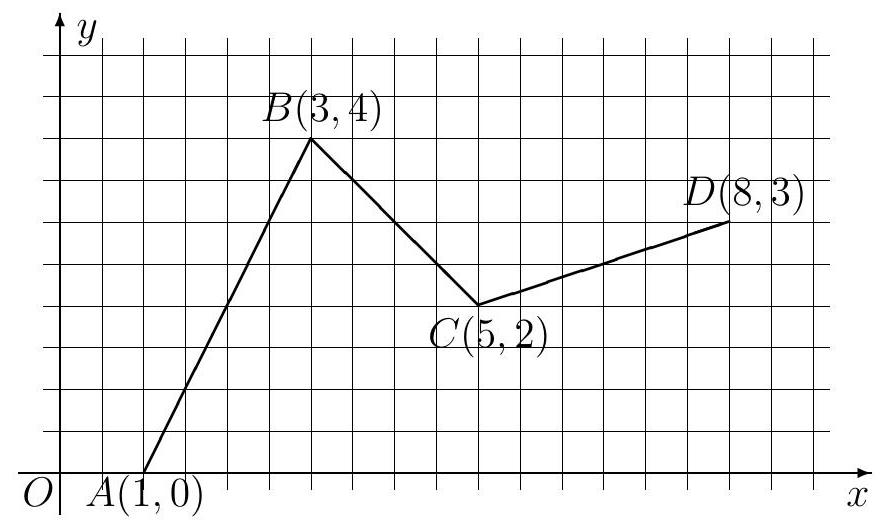
\includegraphics[max width=\textwidth, center]{2024_11_16_c963f0dc5e06cccea777g-05}
  \item Obserwator, stojąc w pewnej odległości, widzi wieżę kościoła pod kątem $60^{\circ}$. Po oddaleniu się o 50 m kąt widzenia zmniejszył się do $45^{\circ}$. Obliczyć cosinus kąta, pod jakim obserwator będzie widział wieżę kościoła, jeśli oddali się o kolejne 50 m .
  \item Wycinek koła ma obwód $2 s$, gdzie $s>0$ jest ustaloną liczbą. Wyrazić pole $P$ tego wycinka jako funkcję promienia $r$ koła. Sporządzić wykres funkcji $P=P(r)$.
\end{enumerate}

\section*{PRACA KONTROLNA nr 3 -POZIOM ROZSZERZONY}
\begin{enumerate}
  \item Sporządzić wykres funkcji $f(m)=\frac{1}{x_{1}}+\frac{1}{x_{2}}$, gdzie $x_{1}, x_{2}$ są pierwiastkami równania $x^{2}-2 m x+m+2=0$, a $m$ jest parametrem rzeczywistym.
  \item Ala ułożyła z czterech klocków liczbę 2009. Następnie spośród tych klocków losowała ze zwracaniem cztery razy po jednym klocku. Jakie jest prawdopodobieństwo, że z otrzymanych w ten sposób cyfr można byłoby utworzyć liczbę:\\
a) podzielną przez 3?\\
b) podzielną przez 4?
  \item Rozważmy funkcje $f(x)=4^{x+1}+4^{2 x+1}+4^{3 x+1}+\ldots$ oraz $g(x)=2^{x}+2^{x-1}+2^{x-2}+\ldots$, gdzie prawe strony wzorów określających obie funkcje są sumami wyrazów nieskończonych ciągów geometrycznych. Wykazać, że funkcja $f(x)$ jest rosnąca. Znaleźć wszystkie liczby $x$, dla których $f(x)=g(x)$.
  \item Rozwiązać nierówność
\end{enumerate}

$$
\frac{\operatorname{tg} x+\sin x}{3 \operatorname{tg} x-2 \sin x} \geqslant \cos ^{2} \frac{x}{2}
$$

\begin{enumerate}
  \setcounter{enumi}{4}
  \item Okrąg styczny do ramion paraboli $y=x^{2}-2 x$ jest styczny równocześnie do osi $O x$. Znaleźć równania stycznych do okręgu w punktach jego styczności z parabolą.
  \item Z odcinków o długościach równych czterem najmniejszym nieparzystym liczbom pierwszym zbudowano trapez, którego pole jest liczbą wymierną. Wyznaczyć tangens kąta między przekątnymi tego trapezu.
\end{enumerate}

\section*{PRACA KONTROLNA nr 4 - POZIOM PODSTAWOWY}
\begin{enumerate}
  \item Mamy dwa termosy kawy z mlekiem. W pierwszym termosie stosunek objętości mleka do objętości kawy wynosi $2: 3$, a w drugim 3:7. Ile litrów płynu należy wziąć z każdego termosu, aby otrzymać 2,4 litra kawy z mlekiem, w której objętość kawy będzie dwa razy większa niż objętość mleka?
  \item Kwotę 100000 zł wpłacono na lokatę roczną, w której odsetki doliczane są co kwartał. Po roku suma odsetek wyniosła dokładnie 4060,401 zł. Znaleźć oprocentowanie tej lokaty. Jakie powinno być oprocentowanie lokaty, aby przy kapitalizacji dokonywanej raz na pół roku osiągnąć ten sam zysk?
  \item Dane sa zbiory $A=\left\{(x, y): x, y, \in \mathbb{R}, y^{2}-4 x^{2} \geqslant 0\right\}$ i $B=\{(x, y):|x|+|y| \leqslant 2\}$. Narysować zbiór $A \cup B$. Znaleźć punkt ze zbioru $A \cup B$ położony najbliżej puntu $C=(3,2)$.
  \item Narysować wykres trójmianu kwadratowego $f(x)=x^{2}+4 x-5$ oraz wykres funkcji $g(x)=4-f(x-2)$.\\
a) Rozwiązać nierówność $f(x)>g(x)$.\\
b) Znaleźć obraz wykresu funkcji $f(x)$ w symetrii względem prostej $x=2$ i na tej podstawie podać wzór tej funkcji.
  \item W ostrosłupie prawidłowym trójkątnym o krawędzi podstawy równej a kąt płaski ściany bocznej przy wierzchołku jest równy $2 \alpha$. Obliczyć objętość tego ostrosłupa oraz sinus kąta nachylenia ściany bocznej do podstawy.
  \item W trapezie $A B C D$, w którym bok $A B$ jest równoległy do boku $D C$, dane są: $\angle B A D=$ $\frac{\pi}{3},|A B|=20,|D C|=8$ oraz $|A D|=5$. Obliczyć obwód tego trapezu, $\sin \angle A D B$ oraz odległość punktu przecięcia się przekątnych tego trapezu od jego podstaw.
\end{enumerate}

\section*{PRACA KONTROLNA nr 4 - POZIOM ROZSZERZONY}
\begin{enumerate}
  \item Dzieląc wielomian $W(x)$ przez dwumian $x-3$ otrzymujemy resztę równą 2 , a dzieląc ten wielomian przez $x-2$ otrzymujemy resztę równą 1 . Wyznaczyć resztę z dzielenia $W(x)$ przez $(x-2)(x-3)$. Znaleźć wielomian trzeciego stopnia spełniający powyższe warunki wiedząc, że $x=1$ jest pierwiastkiem tego wielomianu, a suma wyrazu wolnego i współczynnika przy $x^{3}$ jest równa 0 .
  \item Znaleźć najmniejszą i największą wartość funkcji $f(x)=\sin x-\frac{1}{2} \cos 2 x$ na przedziale $\left[-\frac{\pi}{2}, \frac{\pi}{2}\right]$ i rozwiązać nierówność $-\frac{1}{2} \leqslant f(x) \leqslant \frac{1}{4}$. Zadanie rozwiązać bez używania pojęcia pochodnej.
  \item Rozwiązać nierówność
\end{enumerate}

$$
\log _{\frac{1}{\sqrt{2}}}\left(2^{2 x+1}-16^{x}\right) \geqslant-12 x
$$

\begin{enumerate}
  \setcounter{enumi}{3}
  \item W stożek o kącie rozwarcia równym $2 \alpha$ wpisano kulę o promieniu $R$. Wewnątrz stożka stawiamy na kuli sześcian o maksymalnej objętości i podstawie równoległej do podstawy stożka. Wyznaczyć długość krawędzi tego sześcianu.
  \item Stosunek długości promienia okręgu wpisanego do długości promienia okręgu opisanego na trójkącie prostokątnym wynosi $\frac{1}{3+2 \sqrt{3}}$. Obliczyć sinusy kątów ostrych tego trójkąta.
  \item Ślimak ma do przejścia taśmę o długości 3 metrów zamocowaną w punkcie startu A. W ciągu każdego dnia udaje mu się przejść 1 metr, a każdej nocy gdy śpi, ktoś - ciągnąc za drugi koniec taśmy - wydłuża ją równomiernie o 1 metr. Niech $d_{n}$ oznacza długość taśmy w $n$-tym dniu, a $a_{n}$-odległość ślimaka od punktu A przy końcu $n$-tego dnia.\\
a) Uzasadnić, że ciąg $\left(a_{n}\right)$ zdefiniowany jest następującym wzorem rekurencyjnym: $a_{1}=1$ oraz $a_{n+1}=\frac{3+n}{2+n} a_{n}+1$ dla $n \geqslant 1$.\\
b) Pokazać, że $a_{n}=(n+2)\left(\frac{1}{3}+\frac{1}{4}+\ldots+\frac{1}{n+2}\right), n \geqslant 1$.\\
c) Czy ślimak dojdzie do końca taśmy? Jeżeli tak, to w którym dniu, to znaczy, dla jakich $n$ prawdziwa jest nierówność $a_{n}>d_{n}$ ?
\end{enumerate}

\section*{PRACA KONTROLNA nr 5 - POZIOM PODSTAWOWY}
\begin{enumerate}
  \item Dwie wiewiórki, Kasia i Basia, postanowiły wspólnie zbierać orzechy. Każdego dnia Basia przynosiła do wspólnej spiżarni o 4 orzechy więcej niż Kasia, codziennie tyle samo. Po 30 dniach współpracy wiewiórki pokłóciły się. Basia zostawiła Kasi wszystkie orzechy i założyła własną spiżarnię. Od tamtej pory każda z wiewiórek przynosi do swojej spiżarni tę samą ilość orzechów co przedtem, ale Basia codziennie dostaje 6 orzechów od Kasi. Po 50 dniach samodzielnej pracy Kasia ma jeszcze o 100 orzechów więcej niż Basia. Ustalić, po ile orzechów zbiera codziennie każda z wiewiórek i oszacować, po ilu dniach w spiżarni Basi będzie więcej orzechów niż u koleżanki.
  \item Określić dziedzinę i zbiór wartości funkcji $f(x)=\sin x \cdot \sin 2 x \cdot(\operatorname{tg} x+\operatorname{ctg} x)$. Wykonać staranny wykres funkcji $g(x)=f\left(x-\frac{\pi}{4}\right)+1$ i rozwiązać równanie $g(x)=0$. Posługując się sporządzonym wykresem określić zbiór rozwiązań nierówności $g(x) \geqslant 0$.
  \item Wyznaczyć równania wszystkich prostych, które są styczne jednocześnie do obu okręgów
\end{enumerate}

$$
(x-1)^{2}+(y-1)^{2}=1 \quad \text { oraz } \quad(x-5)^{2}+(y-1)^{2}=1
$$

Obliczenia zilustrować odpowiednim rysunkiem.\\
4. Rozwiązać nierówność

$$
\frac{3 \sqrt{4-x}+1}{1-\sqrt{4-x}}>1-2 \sqrt{4-x}
$$

\begin{enumerate}
  \setcounter{enumi}{4}
  \item Koszt budowy I kondygnacji biurowca wynosi 10 mln zł., a każdej kolejnej jest niższy o 100 tys. zł. od poprzedniej. Planowany koszt wynajmu powierzchni biurowych w tym budynku jest stały do XL kondygnacji i wynosi 200 tys. zł. za całą kondygnację, a potem podwaja się co 5 kondygnacji (na kolejnych 5 kondygnacjach jest stały). Roczny koszt wynajmu ostatniej, najbardziej prestiżowej i droższej od pozostałych kondygnacji jest równy kosztowi budowy całego XXXVII piętra. Oszacować, po ilu latach zwróci się inwestorom koszt budowy tego budynku.
  \item W trapezie równoramiennym kąt przy podstawie ma miarę $\frac{\pi}{3}$, a różnica długości podstaw wynosi 4 . Ustalić, ile powinno wynosić pole tego trapezu, aby można było wpisać w niego koło. W tym przypadku wyznaczyć stosunek pola koła opisanego na tym trapezie do pola koła wpisanego.
\end{enumerate}

\section*{PRACA KONTROLNA nr 5 - POZIOM ROZSZERZONY}
\begin{enumerate}
  \item Znaleźć wszystkie liczby rzeczywiste $m$, dla których równanie
\end{enumerate}

$$
\frac{x}{m}+m=\frac{m}{x}+x+1
$$

ma dwa pierwiastki różnych znaków.\\
2. Rozwiązać nierówność

$$
2^{x^{2}+4}+2^{x^{2}+3}+2^{x^{2}}>5^{x^{2}+1}-25 \cdot 2^{x^{2}-2}
$$

\begin{enumerate}
  \setcounter{enumi}{2}
  \item Określić dziedzinę i zbiór wartości funkcji $f(x)=\operatorname{ctg}(\pi+x) \operatorname{ctg}\left(x-\frac{\pi}{2}\right) \cos x$. Sporządzić staranny wykres funkcji $g(x)=2 f\left(\left|x-\frac{\pi}{4}\right|\right)-1$. Na podstawie wykresu i niezbędnych obliczeń rozwiązać nierówność $g(x) \leqslant-2$, a zbiór jej rozwiązań zaznaczyć na osi OX.
  \item Rozwiązać nierówność
\end{enumerate}

$$
\log _{x^{2}}(3 x-1)-\log _{x^{2}}(x-1)^{2}+\log _{x^{2}}|x-1| \geqslant \frac{1}{2}
$$

\begin{enumerate}
  \setcounter{enumi}{4}
  \item W ostrosłupie sześciokątnym prawidłowym kąt dwuścienny utworzony przez płaszczyzny przeciwległych ścian bocznych ma miare $\frac{\pi}{4}$. Wyznaczyć promień $R$ kuli opisanej na tym ostrosłupie jako funkcję długości $a$ boku jego podstawy.
  \item W koło wpisano ośmiokąt foremny, w ośmiokąt koło, w koło kolejny ośmiokąt foremny itd. Wysunąć hipotezę o wartości pola $n$-tego koła i uzasadnić ją indukcyjnie. Suma pól nieskończonego ciągu kół otrzymanych w ten sposób jest ośmiokrotnością pola jednego z nich. Ustalić którego, nie stosując obliczeń przybliżonych.
\end{enumerate}

\section*{PRACA KONTROLNA nr 6 - POZIOM PODSTAWOWY}
\begin{enumerate}
  \item Logarytmy (przy ustalonej podstawie) z liczb: $a_{1}=\frac{2}{5} x, a_{2}=x-1, a_{3}=x+3$ tworzą ciąg arytmetyczny. Wyznaczyć $x$. Dla znalezionego $x$ obliczyć sumę początkowych dziesięciu wyrazów ciągu geometrycznego, którego trzema pierwszymi wyrazami są liczby $a_{1}, a_{2}, a_{3}$.
  \item Odcinek o końcach $A\left(\frac{5}{2}, \frac{\sqrt{3}}{2}\right), B\left(\frac{5}{2}, \frac{3 \sqrt{3}}{2}\right)$ jest bokiem wielokąta foremnego wpisanego w okrąg styczny do osi $O x$. Wyznaczyć równanie tego okręgu i współrzędne pozostałych wierzchołków wielokąta. Ile rozwiązań ma to zadanie? Sporządzić rysunek.
  \item Dany jest ostrosłup prawidłowy trójkątny, w którym krawędź boczna jest dwa razy dłuższa niż krawędź podstawy. Ostrosłup ten podzielono płaszczyzną przechodzącą przez krawędź podstawy na dwie bryły o tej samej objętości. Wyznaczyć tangens kąta nachylenia tej płaszczyzny do płaszczyzny podstawy. Sporządzić rysunek.
  \item O kącie $\alpha$ wiadomo, że $\sin \alpha-\cos \alpha=\frac{2}{\sqrt{3}}$.\\
a) Określić, w której ćwiartce jest kąt $\alpha$.\\
b) Obliczyć $\operatorname{tg} \alpha+\operatorname{ctg} \alpha$ oraz $\sin \alpha+\cos \alpha$.\\
c) Wyznaczyć $\operatorname{tg} \alpha$.
  \item Dłuższa przyprostokątna $b$ trójkąta prostokątnego o kącie ostrym $30^{\circ}$ jest średnicą półokręgu dzielącego ten trójkąt na dwa obszary. Wyznaczyć stosunek pól tych obszarów oraz długość promienia okręgu wpisanego w obszar zawierający wierzchołek kąta $60^{\circ}$. Sporządzić rysunek.
  \item Dwaj turyści wyruszyli jednocześnie: jeden z punktu $A$ do punktu $B$, drugi - z $B$ do $A$. Każdy z nich szedł ze stałą prędkością i dotarłszy do mety, natychmiast ruszał w drogę powrotną. Pierwszy raz minęli się w odległości 12 km od punktu $B$, drugi - po upływie 6 godzin od momentu pierwszego spotkania - w odległości 6 km od punktu $A$. Obliczyć odległość punktów $A$ i $B$ i prędkości, z jakimi poruszali się turyści.
\end{enumerate}

\section*{PRACA KONTROLNA nr 6 - POZIOM ROZSZERZONY}
\begin{enumerate}
  \item Rozwiązać równanie
\end{enumerate}

$$
\sqrt{x^{2}-3}+\sqrt{5-2 x}=4-x
$$

\begin{enumerate}
  \setcounter{enumi}{1}
  \item Z urny zawierającej 2 kule białe, 4 czerwone i 3 czarne wylosowano jedną kulę. Następnie wylosowano jeszcze trzy kule, gdy pierwsza okazała się biała, dwie kule, gdy pierwsza była czerwona, lub jedną kulę, gdy w pierwszym losowaniu wypadła czarna. Obliczyć prawdopodobieństwo, że w urnie nie pozostała żadna kula biała.
  \item Podstawą graniastosłupa prostego jest trójkąt o bokach $a, b$ i kącie między nimi $\alpha$, a przekątne ścian bocznych, wychodzące z wierzchołka kąta $\alpha$, są do siebie prostopadłe. Obliczyć objętość graniastosłupa.
  \item Na jednym rysunku sporządzić staranne wykresy funkcji
\end{enumerate}

$$
f(x)=\sqrt{6 x-x^{2}} \quad \text { oraz } \quad g(x)=\left|\frac{3}{2}-f(x+2)\right|
$$

Obliczyć pole figury ograniczonej wykresem funkcji $g(x)$ i osią $O x$.\\
5. Podać dziedzinę i sprawdzić tożsamość

$$
\operatorname{tg}^{2} \frac{\alpha}{2}=\frac{1-\cos \alpha}{1+\cos \alpha}
$$

Cosinus kąta ostrego $\alpha$ wynosi $\frac{1}{8}$. Korzystając z powyższej tożsamości, obliczyć wartość sumy $\operatorname{tg} \frac{\alpha}{4}+\operatorname{tg} \frac{\alpha}{2}+\operatorname{tg} \frac{3 \alpha}{4}+\operatorname{tg} \alpha$. Wynik podać w najprostszej postaci.\\
6. Punkt $C(-2,-1)$ jest wierzchołkiem trójkąta równoramiennego $A B C$, w którym $|A C|=$ $|B C|$. Środkowe trójkąta przecinają się w punkcie $M(1,2)$, a dwusieczne w punkcie $S\left(\frac{1}{2}, \frac{3}{2}\right)$. Wyznaczyć współrzędne wierzchołków $A$ i $B$.


\end{document}